\subsection{Gen Phase}
\label{sec:gen}

The Gen phase accepts an input dataset of line segments $N$ and starts by partitioning the input across the worker nodes in a distributed cluster using a global quadtree spatial index.
Each data partition $P_i$ covers a specific spatial area represented by its minimum bounding rectangle (MBR) $B_i$.
Figure~\ref{fig:ddcel:input} shows an example of four leaf nodes of a quadtree built for input spatial line segments. Solid lines represent the line segments, and dashed lines represent the partitions' MBRs.

\begin{figure}[tb]
	\centering
	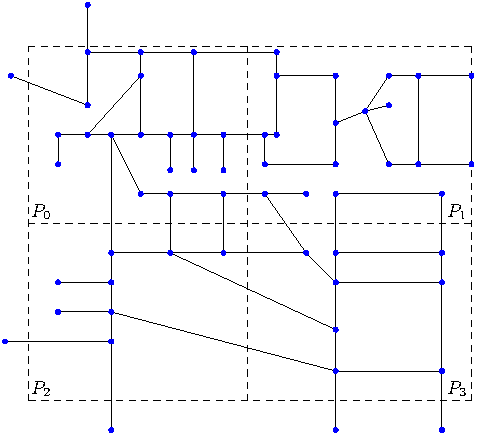
\includegraphics[width=0.75 \linewidth ]{chapter2/model/input-network}
	\caption{Partitioned input spatial lines.}
	\label{fig:ddcel:input}
\end{figure}

After spatially partitioning the input lines, each partition generates its vertices, half-edges, and faces (collectively the partition DCEL) using the subset of the dataset that intersects with the partition's MBR.
The \textit{partition vertices} are the vertices that are wholly contained within the partition MBR. 
On the other hand, the \textit{partition half-edges} are any half-edge that intersects with the partition MBR.
\textit{Partition faces} are the faces that are wholly contained within the MBR of the partition.
On each data partition $P_i$, the Gen phase undergoes four main procedures; 
(1) first, generating the partition vertices and half-edges, 
(2) second, marking the dangle half-edges, 
(3) third, setting the next half-edge pointers for all half-edges and marking the cut edges, 
(4) lastly, generating the partition faces. 

\vspace{4pt}
\textit{\textbf{Step 1: Generating the Partition Vertices and Half-edges.}}
\\
In the first step, the Gen Phase starts with populating the vertices and the half-edges RDDs of the DCEL data structure.
Each partition $P_i$ receives a subset of the input dataset that intersects with the partition's boundary.
For every line segment object $o$ received at partition $P_i$ ($o \in P_i$), two vertices are generated ($v_1$, $v_2$); one for each endpoint on this line segment ($p_1$, $p_2$). These two vertices objects ($v_1, v_2$) are appended to the vertices RDD in the DCEL data structure.
We also generate two half-edges ($h_1, h_2$) for every line segment. 
The first half-edge $h_1$ has its destination vertex $v_1$, while the other half-edge $h_2$ has its destination vertex $v_2$. These two half-edges are assigned as twins.
The half-edge $h_1$ is appended to the incident list of the vertex $v_1$. Similarly, $h_2$ is appended to $v_2$'s incident list.
For a half-edge to span multiple partitions, we check whether it is wholly contained within the partition MBR $B_i$; if not, and it is just intersecting, then this half-edge spans multiple partitions. 
These half-edges are duplicated on all partitions they intersect with.
The remaining attributes of each half-edge object are assigned in the subsequent steps. 
The two generated half-edge objects ($h_1, h_2$) are appended to the half-edges RDD in the DCEL data structure.
Figure \ref{fig:ddcel:step1} shows a graphical illustration of the DCEL data structure representing the input lines after generating the vertices and the 
half-edges on all data partitions.

\begin{figure}[tb]
	\centering
	
\includegraphics[width=0.75 \linewidth ]{chapter2/model/ddcel-1}
	\caption{DCEL vertices and half-edges.}
	\label{fig:ddcel:step1}
\end{figure}


\vspace{4pt}
\textit{\textbf{Step 2: Marking the Dangle Half-edges.}}
\\
Dangle half-edges are not part of any face; thus, marking them is essential to exclude them during the polygonization procedure. To find dangles in the input lines, we use previously generated information, i.e., information about the vertices and their incident half-edges. 
We compute the degree of each vertex $v \in V$ populated in the previous step. A vertex degree is the number of non-dangle half-edges in its incident half-edges list. If the degree of an arbitrary vertex $v$ is less than or equal to 1 ($degree(v) \le 1$), then all of $v$'s incident half-edges and their twins are also dangle half-edges. 
Marking any new half-edge as a dangle requires recomputing the degree of the vertices connected to it. 
Thus, marking the dangle half-edges is an iterative process. After the initial run over all vertices and marking the initial dangle half-edges, we reiterate over the vertices to check for newly found dangle half-edges. We keep iterating until convergence when no new dangle half-edges are detected.


\vspace{4pt}
\textit{\textbf{Step 3: Setting the Half-edges' Next Pointers, and Marking the Cut Edges.}}
\\
The third step is divided into three smaller steps: (a) setting the next half-edge pointer for each half-edge, (b) marking the cut edges, and (c) updating the next half-edges accordingly.
To set the next pointer for each half-edge, we use information from the previous two steps, i.e., the vertices incident half-edges and the current dangle half-edges.
For each vertex $v \in V$, we sort its incident half-edges list in clockwise order, excluding the dangle half-edges. 
After sorting the incident half-edges list $v.incidentH$, for every pair of half-edges $v.incidentH[t]$, $v.incidentH[t+1]$ in the sorted list, we assign $v.incidentH[t].next$ to $v.incidentH[t+1].twin$. For the last incident half-edge in the sorted list $v.incidentH[v.incidentH.len-1]$, we assign its next half-edge to $v.incidentH[0].twin$.


After the initial assignment of the next half-edge pointers, we proceed with the second sub-step, marking the cut edges.
To mark the cut edges, we start our procedure at an arbitrary half-edge $h_{initial}$ and assign our $h_{current}$ half-edge pointer to it. We advance the $h_{current}$ pointer at each iteration to the $h_{current}$'s next ($h_{current} = h_{current}.next$), storing all visited half-edges in a list (current cycle). We keep advancing the $h_{current}$ pointer till we reach one of three cases.
(1) We return to the initial half-edge $h_{initial}$, which means a cycle is detected and no cut edge is detected.
(2) The half-edge $h_{current}.next$ is not available, which also means no cut edge is detected.
(3) We find $h_{current}.twin$ in the current cycle, which means that $h_{current}$ and its twin are both cut edges. 
Once we reach one of these cases, we mark all visited half-edges as such and proceed with a new arbitrary half-edge to be $h_{initial}$.
This process is terminated when all the partition half-edges are visited.

In the third sub-step, after marking all cut edges, we update the next pointers while excluding the cut edges. 
For each vertex $v \in V$, we sort its incident half-edges list in clockwise order again, now while excluding both the dangle and the cut edge half-edges.
After sorting the incident half-edges list $v.incidentH$, we re-execute the same process of the first sub-step, assigning $v.incidentH[t].next$ to $v.incidentH[t+1].twin$. 
Figure~\ref{fig:ddcel:step2} shows the DCEL data structure after removing the dangle and cut edges.


\begin{figure}[tb]
	\centering
	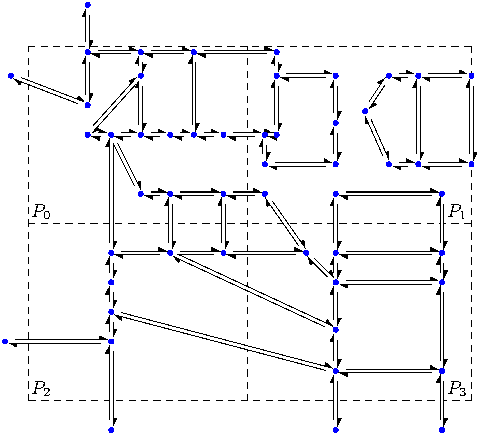
\includegraphics[width=0.75 \linewidth ]{chapter2/model/ddcel-2}
	\caption{DCEL vertices and half-edges after dangle and cut edge removal.}
	\label{fig:ddcel:step2}
\end{figure}

\vspace{4pt}
\textit{\textbf{Step 4: Generating the Partition Faces.}}
\\
Polygonization on each partition $P_i$ starts with selecting an arbitrary half-edge as our initial half-edge $h_{initial}$.
We initially assign our $h_{current}$ half-edge pointer to $h_{initial}$. We advance the $h_{current}$ pointer at each iteration to the $h_{current}$'s next ($h_{current} = h_{current}.next$), storing all visited half-edges in a list $cycle$. We keep advancing the $h_{current}$ pointer till we reach one of the following cases:
(1) We return to the initial half-edge $h_{initial}$, which means that we have found a face. In this case, we add the found face $f$ to the faces collection $F_0$ and assign $h.incidentF = f, \;\; \forall h \in cycle$.
(2) The $h_{current}.next$ is not available, and $h_{current}$ is a half-edge that spans multiple partitions. In this case, the cycle needs more information from the neighboring partitions to be completed, and the current partition's data is insufficient to produce this face.
To complete this cycle, we either pass the incomplete cycle into the Rem phase (the current list $cycle$), where it collects all incomplete cycles from all partitions and attempts to join them to form a face. Another approach would be passing the plain half-edges in this cycle to the next phase. Both approaches are discussed in detail in Section~\ref{sec:rem}.
Once we finish processing this cycle, we mark all visited half-edges as such, clear the cycle, and proceed with a new arbitrary half-edge to be $h_{initial}$.
This process is terminated when all the partition half-edges are visited.
In Figure~\ref{fig:ddcel:faces}, the dotted faces are the faces generated in this phase (Gen Phase).

\begin{figure}[tb]
	\centering
	
\includegraphics[width=0.75 \linewidth ]{chapter2/model/ddcel-3}
	\caption{DCEL faces.}
	\label{fig:ddcel:faces}
\end{figure}
